% {{{ Preamble
\documentclass[pdftex,12pt,a4papaer]{report}
\usepackage[pdftex]{graphicx}
\usepackage{fancyhdr}
\usepackage{parskip}
\usepackage[numbers]{natbib}
\usepackage{url}
\usepackage{amsmath}
\usepackage{amsfonts}
\usepackage{setspace}
\usepackage{paralist}
\usepackage[]{units}
\usepackage{tabto}
\usepackage{float}
\usepackage{comment}
\usepackage{titling}
\usepackage{hyperref}
\usepackage{todonotes}
\usepackage{textcomp}
% \usepackage{minted}
\pagestyle{fancy}
% }}}
\setlength{\marginparwidth}{3cm}

\linespread{1.5}

\title{DRACL 2.0 Proposal}
\author{Steven Allen}
\date{\today}

% {{{ Header
\rhead{\thedate}
\chead{\thetitle}
\lhead{\theauthor}
% }}}

\newcommand{\note}[1]{\textit{\textbf{Note:} #1}}

\begin{document}

\thispagestyle{plain}

\begin{center}
    \vspace*{\fill}
    {%
        \onehalfspacing{} \bfseries \Large
        DRACL (Decentralized Resource Access Control List) \\
    }

    \vspace{\fill}
    {\large
    \begin{minipage}{0.9\textwidth}
        \emph{Author:} \theauthor{} \hfill \emph{Advisor:} David Karger
        \\
        \begin{center}
              \thedate{}
        \end{center}
    \end{minipage}
    }
    \vspace*{\fill}
\end{center}

\tableofcontents

\newpage

\chapter{Introduction} 

DRACL is a federated, privacy-preserving access control system that allows
content publishers (not necessarily the professional kind) to control access to
content hosted on services (content hosts) by providing these services with
access control lists (ACLs) that opaquely specify which consumers and groups of
consumers should be granted access. Unlike existing solutions, DRACL does not
rely on a centralized authority (unlike Facebook Connect, Google), does not
allow access control providers to masquerade as their users\note{Consumers and
  producers. should I fix this use?} (unlike Mozilla
Persona, OpenID), and allows publishers to share content with their friends on
third party content hosts without revealing their social networks to these
content hosts.

\section{Terms}

For convenience, we define the following terms:

\begin{compactdesc}
    \item[Identity] An assumed identity. That is, identities may not correspond
      one-to-one to real people. They may be pseudonymous, or may correspond to
      a group of people.
    \item[Publisher] A user that publishes content and wishes to control
      access to said content.
    \item[Consumer] A user that accesses content published by a publisher
      with the publisher's permission.
    \item[Authorized Consumer] A consumer that is authorized to access a
      particular resource.
    \item[Group] A group of users as defined a publisher. In DRACL, groups
      are the unit of access control (i.e., publishers grant access to
      groups, not directly to individual consumers).
    \item[Access Control Provider (AP)] A helper service for facilitating
      access control. Every DRACL user\note{again, that word} will have an AP (just like every email
      user has an email provider). Basically, the AP can perform limited actions on
      behalf of users while offline and can help ensure that a compromise of a user's
      account is recoverable.
    \item[Content Host] A party using this system to authenticate content it
      hosts. For example, Flicker, Facebook, Imgur, etc.
    \item[Friend] Same as a Facebook friend. That is, the relationship may or
      may not be friendly.
\end{compactdesc}

\section{Requirements}

\note{David: I can't discuss Facebook etc. without first specifying a criteria
by which to judge them. However, I've expanded this section to discuss why we
care about our requirements and changed it to avoid actually talking about
DRACL.}

We would like a practical, secure, privacy preserving, and developer and user
friendly access control system for the web. In this section, we discuss what
these requirements mean in the context of access control systems and why we care
about them. Additionally, we make no assumptions about whether or not such a
system already exists; we simply state what we want out of such a system.

Two explicit non-goals are hiding the content from content hosts and hiding
social networks from global adversaries. We want an access control system, not a
full-fledged privacy preserving communication system.

TODO: EXPLAIN! ^^

% Finally, due to some privacy/efficiency/security trade-offs we've made, we
% couldn't hide the identity of publishers (anonymous publishing) or hide
% publishers' social networks from their access control providers.

\subsection{Practical}

By practical, we mean a good access control system should be designed to work in
the world as it is, not as we wish it were.

For example, it shouldn't assume that publishers will run their own servers or
pay for anything for that matter. The amount of invasive advertising, poor
software, and privacy violations people tend to put up with on the internet for
``free'' services is a testament to how far people will go to avoid paying.

Additionally, it can't assume that anyone can build a perfect implementation. No
practical, complex system can hope to achieve perfect security and perfect
uptime. At the end of the day, this system will be built and maintained by
humans so we must design it with that in mind.

Finally, such a system should keep any work done by any third parties to a
minimum. This is a direct result of users not being willing to pay for anything:
nobody can't afford to run overly expensive computations on behalf of users for
free.

\subsection{Secure}

By secure, we mean that publishers should be able to efficiently/reliably revoke
access from consumers, compromises should be recoverable, and only authorized
consumers should be able to access content.

First, for efficient and reliable revocation, a publisher should not have to
contact every content host in order to revoke access to some piece of content.
First, this would trigger a lot of up-front network traffic, even for old
content that may never be accessed again. Second, it would violate the fail-safe
principle of systems design: if a publisher were unable to contact some of their
content hosts for some reason, there would be no way to revoke access.

Second, no compromise of any single party should be unrecoverable and no
compromise of any single party should bring down the entire system. Websites are
hacked all the time and user account compromise is common so any system that
can't recover from compromise is dead in the water.

Finally, only authorized consumers should be able to access content, no trusted
third parties. Currently, if someone were to hack Gmail, they'd be able to
access pretty much everything on the public internet (through, e.g., password
reset emails). This was a mistake. From a security perspective, it's terrifying;
from a business perspective, it's a unacceptable liability. No sane,
well-intentioned party wants that much power; this is why Facebook, Google, etc.
are pushing for end-to-end encryption. Therefore, a good access control system
should avoid this problem by design.

\subsection{Privacy Preserving}

By privacy preserving we mean that a good access control system should avoid
revealing metadata. That is, it should reveal neither the identities of
consumers nor the composition of its publishers' social networks when possible.

First, such a system should not reveal the identities of consumers to content
hosts because people should not be excluded from social interactions for valuing
their privacy. In the web as it exists today, it's impossible to participate in
social networks without handing out personal information to third parties. This
forces people to either hand out this information or isolate themselves
completely. While, to prevent abuse, social networks often need
publishers/publishers to identify themselves, we believe that consumers should
be able to access content without identifying themselves. This would allow
people to anonymously access content on any content host while only publishing
content on content hosts they trust.

Second, such a system should not reveal the identities of consumers to content
hosts because people should be free to associate without being judged by
association. That is, it's a violation of Alice's privacy for Betty to publicly
declare an association with Alice (implicitly or explicitly) without her
consent. For example, if Betty, Carol, Dora, and Ester are all known members of
a local pregnancy group, them all claiming an association with Alice is a good
indication that she is also pregnant. This isn't just an abstract issue;
information like this is very valuable to advertisers. There have been
documented incidents~\cite{target} of advertisers accidentally outing pregnant
teens to their parents by sending them advertisements targeted at pregnant
women.

Third, such a system should not reveal the structure of a publisher's social
network, \emph{especially} to members of their social network, because
encourages publishers to share more openly than they might feel comfortable
doing\todo{not the best way of putting this}. People should feel free to exclude
others from their social network; the ability to communicate privately (exclude
unwanted parties) is necessary to prevent self-censorship. For example, a good
access control system should not reveal that two consumers are members of some
shared group while a third consumer is not. This could pressure the publisher to
include all three in the same group to avoid offending the third would, in turn,
cause the publisher to either share content more widely than they might
otherwise want or refrain from sharing at all (a chilling effect).

% Unfortunately, this goal isn't entirely achievable in a practical system due to
% security and efficiency trade-offs but DRACL gets pretty close. See section
% the discussion section on privacy (section \ref{sec:privacy}) for details on what we
% actually achieved.

% TODO: Uncomment?/move How do I deal with comments like this?

\subsection{Developer Friendly}
\label{sub:goal-developer}

By developer friendly, we mean that a good access control system should be at
least as easy to deploy as a custom password-based identity scheme (the current
de facto standard), it shouldn't require significant infrastructure changes, and
it should make it easier to bootstrap new content host.

We believe that a lack of developer friendliness contributed significantly to
the failure of systems like OpenID\cite{openid}. More concretely, we know that
the difficulty to deploy and maintain SSL certificates has been a significant
barrier to adoption of SSL as demonstrated by the rapid rise --- 5\% in 6 months
--- of SSL deployment after the launch of Let's Encrypt~\cite{lets-encrypt}.

Furthermore, developers should \emph{want} to use this access control system
because it can help developers avoid the bootstrap problem. In the web as-is,
you need users to attract users because nobody wants to be alone on a content
host. A good global access control system should help alleviate this problem by
allowing users to access content on any content host without having to even so
much as login.

\subsection{User Friendly}
\label{sub:goal-user}

By user friendly, we mean that a good access control system should make the
internet look like one interconnected social network. Users shouldn't have to
manage multiple sets of credentials or manually recreate their social network on
every content host they use.

Currently, content hosts (usually) force their users to manage one set of
credentials per service. In addition to being beyond annoying, this practice
encourages users to choose simple passwords or reuse them. A good global access
control system can eliminate this problem by allowing users to manage a single
access control account and re-use the same account from service to service.

Additionally, it's prohibitively difficult to move between content hosts because
because social networks are usually tied to a single content host. A global
access control system can alleviate this problem by allowing publishers to
grant access to their friends on any content host regardless of what content
hosts their friends use.

Finally, a consequence of making it easier to move between content hosts is
more practical competition. Competition is not only good for users, it's
absolutely necessary to keep companies from screwing their users over in pursuit
of more money. See AT\&T\texttrademark{}\cite{att} policy and
Comcast's\texttrademark{}\cite{comcast} recent attempt to charge an additional
fee for not snooping on their customers browser history.

\section{Existing Systems} 

Given the goals stated in the previous section, this section explores existing
systems and motivates the need for a new one.

\subsection{Bearer Credentials}

Before going into real access control systems, we need to mention an obvious
solution: bearer credentials. You've almost definitely run across them, usually
in the form of ``secret'' links. That is, if you know the link, you can access
the resource.

One could conceivably build an entire access control system out of bearer
credentials. Unfortunately, most bearer credentials provide no simple way of
revoking access; you can't just take back a link. They also tend to be easy to
lose or accidentally give away (i.e., make public).

Some systems like Google's Macaroons~\cite{macaroon} fix these problems by
issuing short-lived bearer credentials that can optionally require the bearer to
prove knowledge of some additional key. Macaroons even support delegation.
However, being short lived, we'd still need to design a system for issuing and
managing Macaroons.

In short, bearer credentials are a useful component of access control systems
but don't really solve the problem.

\subsection{Identity Systems}

The most common access control scheme is to assign one or more unique identities
to all users and then have all content hosts record which identities have access
to what. We call these identity systems because, while access control systems
can be built on top of them, they don't inherently provide access control as a
feature.

This type of system is inherently bad for privacy because content hosts learn
the identities of who has access to what and, by extension, who knows who. While
this privacy issue sufficiently motivates an alternative design, we have
included this section to give an overview of some common existing systems and to
learn from their shortcomings (in addition to the privacy problem).

\subsubsection{Site Specific Identity}

The vast majority of content hosts today force users to create site-specific
accounts. This is a poor solution to the access control problem for both users
and content hosts because it introduces security hazards and has poor developer
and user usability. The only goal this system meets is that no unauthorized
third party can access a publishers content. It's also arguable that it
meets the goal of not revealing the publishers social network to consumers
but there's no guarantee about this and content hosts don't always get this
right (e.g., the Google Buzz~\cite{google-buzz} fiasco).

From a user usability standpoint, site-specific accounts force users to create new
accounts and replicate their social networks on every content host they use. As
discussed in the goals section on user friendliness (section \ref{sub:goal-user}), this is
bad for usability.

% DRACL avoids the first problem by allowing users to create a single account with
% a single Access Control Provider for use on multiple content hosts. It avoids
% the second problem by handling access control on behalf of the content host.

From a developer usability standpoint, site-specific accounts force content
hosts to implement custom account/access control systems and make it harder to
attract new users because developers have to convince new users to ``sign up''
before they can participate. Again, refer the goals (subsection \ref{sub:goal-developer}) for
why this is a problem.

% DRACL solves the first problem by allowing content hosts to
% focus on whether or not an operation should be permitted instead of messing
% around with identities.

Site specific accounts are a security hazard because content hosts are
notoriously bad at safely storing credentials and users are notoriously bad at
choosing/remembering safe passwords. For example, content hosts often store user
credentials in the clear~\cite{plaintext} and users often reuse passwords and/or
use weak passwords~\cite{ms-passwords}.

% DRACL reduces these security hazards by restricting credential checking to APs
% and reducing the number of credentials that users have to manage to one (the one
% they need to authenticate to their AP).

\subsubsection{Centralized Identity}

Centralized identity systems, such as those provided by Google and Facebook,
allow users to identify to multiple sites using a single set of credentials.
These systems therefore solve all of the security problems we mentioned in the
site specific password section as users only have one set of credentials managed
by a single, hopefully competent, entity. They also solve the associated
usability problem of users having to remember multiple passwords.

While centralized identity systems sometimes increase usability by allowing
users to carry their social networks with them to content hosts (e.g. Facebook),
they can't provide a way to do so while maintaining privacy. That is, for one
user to allow another user to access a resource on a content host, the first
user must identify the second user to the content host. This is a fundamental
problem with identity systems because they operate on the level of identity.

Again, because these systems operate on identities, they force content hosts to
implement their own access control systems which, again, violates our stated
goals. Content hosts shouldn't have to reinvent the wheel.

Finally, because these systems are centralized, users are forced to choose
between a few ``accepted'' providers and can't run their their own and content
hosts are forced to support whatever identity systems happen to be in vogue at
the time.\todo{This should probably also be mentioned in the goals. Does it go
under privacy or user friendly?}

\subsubsection{Decentralized Identity}

Decentralized identity systems such as OpenID~\cite{openid},
Persona~\cite{persona}, and WebID~\cite{webid} allow users to identify to
multiple services using the same credentials but, unlike centralized identity
systems, decentralized identity systems do not force users to choose between a
few ``accepted'' providers. Additionally, in theory, content hosts should be
able to support exactly one decentralized identity system --- assuming they
eventually converge. While decentralized identity systems address the user
choice concern, they still don't address our privacy concerns because they still
operate on the level of identity.

\subsection{Access Control Systems}

Unlike identity systems, access control systems directly dictate what operations
a system should and should not permit. Where an identity system answers the
question ``Does <PROOF> imply that <CLIENT> is <IDENTITY>?'', access control systems
answer the question ``Does <PROOF> imply that <CLIENT> has <PERMISSION>?''. In our
case, ``<PERMISSION>'' is usually ``can access <CONTENT>''. This categorically
addresses our usability concerns with identity systems because the entire social
network is now defined in by a unified system. Unfortunately, there aren't any
existing access control systems that address our privacy and security concerns.

\subsubsection{Centralized Access Control}

Centralized access control systems such as Kerberos~\cite{kerberos} and
LDAP~\cite{ldap} allow services to offload user/group management to third
parties (the access control provider). While, as noted above, this solves the
usability problems in centralized identity systems, it makes the centralization
problem much worse. While content hosts can allow different users to
authenticate with different centralized authentication services, they cannot
allow users to choose their own centralized access control service without
partitioning the social network because, by definition, centralized access
control services don't interoperate.

\subsubsection{Decentralised Access Control}

Decentralized (federated, really) access control systems offer the same benefits
as centralized access control systems but without the drawbacks of being a
centralized system. That is, users can freely choose between providers or run
their own. Thus, decentralized access control systems categorically meet our
user friendliness goals.

There are existing decentralized access control systems such as \cite{attrib}
\cite{privattrib} \cite{drbac} \cite{socnet} and the Kerberos Consortium's User
Managed Access (UMA)~\cite{uma}. Unfortunately, while both \cite{attrib} and
\cite{privattrib} describe cryptographic protocols for privacy preserving
decentralized access control, neither attempt to design an implementable system.
UMA\cite{uma} \cite{drbac} and \cite{socnet} provide a more thorough system
designs (UMA even provides a system specification) but they (1) fail to even
address the question of user privacy and (2) completely trust a third party
access control provider (e.g., UMA).

Now we're in uncharted territory. So far, we've decided that we need an access
control system, not an identity system, and would like it to be decentralized.
Next, we'll delve into the decentralized access control design space and work
our way towards a design that satisfies our goals.

\section{Design}
\label{sec:design}

Now that we've determined that we need a decentralized access control protocol,
this section explores the design space and works towards the final design of
DRACL. If you just want to know how DRACL works but not why or how we got there,
proceed to the Design Overview (chapter \ref{chap:design-overview}) for a
top-down view of the DRACL protocol.

\subsection{Zeroth Attempt}

The brain-dead solution is to have content hosts ask publishers directly if
consumer should be able to access some content. This obviously won't work
because we can't expect the publisher's computer to be online all the time. As a
matter of fact, for all we know, the publisher may never come back online ---
they could be dead.

\subsection{First Attempt}

The first reasonable design would be to have every publisher pick an access
control provider (AP) and have their AP act their behalf to handle all access
control decisions in real-time. Basically, when publishing content, publishers
would also assign a content ID (CID) to the content in question and tell the
content host: when a consumer tries to access the content identified by CID, ask
AP if they should be granted access. The user would then tell their which
consumers and/or groups of consumers should be granted access to the content
identified by CID.

On the plus side, this is an extremely simple system and meets many of our
goals. From a privacy standpoint, neither consumers nor content hosts learn
anything about publishers' social networks. From a security standpoint access
can be revoked without contacting individual content hosts and compromise 
is all recoverable as nobody stores any security-sensitive state. From a
developer friendliness standpoint, this system is great because it's simple.
Unfortunately, this has has a some major drawbacks.

\subsection{Don't Be A Weapon}

For one, content hosts have to make network requests on behalf of clients to
servers specified by clients. From a security standpoint, this very bad as it
opens up the content host to resource exhaustion attacks and makes it possible
to use the content host in DDoS attacks. For the resource exhaustion attack, an
attacker could repeatedly cause a content host to attempt to contact
non-responsive AP servers causing the content host to quickly run out of kernel
resources resources. For DDoS attacks, an attacker could use a large number
content hosts to saturate a single AP server's resources. From the access
control server's standpoint, this traffic would be indistinguishable from
legitimate traffic so it couldn't protect itself.

There's a simple solution: have the consumer contact the AP on behalf of the
content host. That is, the content host asks the consumer's browser to present a
certificate from the AP certifying that the user should be able to access the
content identified by the CID. The consumers browser then authenticates to the
AP, gets the certificate, and returns it to the content host. As a matter of
fact, most access control services, including the Kerberos Consortium's User
Managed Access (UMA)~\cite{uma}, operate this way.

%Unfortunately, by introducing crypto into the protocol, we've made it
%significantly harder to recover from system compromise violating our no
%compromise of any single party should be unrecoverable requirement. In the ``first
%attempt'' protocol, there were no secrets --- not in the protocol itself, at
%least. However, by adding crypto, we've introduced secrets. Now, if these
%secrets are leaked, we'll need a way to invalidate them. We'll fix this later
%but you should keep it in mind.

\subsection{Distribute The Storage}

Unfortunately, there's another problem with this system as described: the access
control server needs to keep track of every piece of content ever published.
This means that the AP's state will grow linearly with the amount of content
published.

Our solution to this was to replace the CIDs with access control lists (ACLs)
encrypted with a key known to the AP. Now, instead of asking the AP if a user
should be granted access to a piece of content, the content host asks the AP if
a user is a listed in an ACL (or is a member of a group listed in the ACL).
Basically, we're just distributing the load by storing the ACL on the content
hosts instead of AP and using cryptography to make sure no party learns anything
they shouldn't.

\subsection{Don't Trust Third Parties}

At this point, our system is looking pretty good but we still haven't addressed
a key goal: no third parties with perfect security or uptime requirements. In
the system as described so far, we fully trust that APs cannot be compromised;
compromising the AP compromises the entire system (well, all users of that AP at
least). Ideally, we want some sort of black-box that only hands out
authorizations to the correct consumers but having every publisher ship a
literal black-box to their APs is obviously impractical. However, there's a
better way: cryptography, specifically functional encryption.

Using some fancy crypto, publishers can give their APs virtual black boxes that,
given user ID and a specially constructed ACL, can construct a certificate
usable only by the given consumer --- using some consumer-specific secret ---
if, and only if, they a member of the ACL. Unfortunately, this isn't without
drawbacks: this crypto is \emph{very} computationally expensive --- on the order
of a second of CPU time. We've exchanged ``no expensive computation by third
parties'' for ``no third parties with perfect security requirements''.

\subsection{Distribute The Load}

However, we can now kill two birds with one stone by giving these black boxes to
consumers, instead of APs, cutting the APs out of the picture entirely. By doing
this, we've moved the heavy crypto from the access control provider to the
consumer and made it possible for the consumer to authenticate against multiple
ACLs without having to contact the AP each time.

However, now we can't remove users from groups. Basically, if one of these black
boxes thinks a user is in a group, it will give this user certificates granting
them access to ACLs that list that group. Unfortunately, after we've given this
black box to a consumer, we can't reach into the consumer machine and remove the
black box.

This time, we can solve this by making the black boxes expire after a period of
time. That way, while publishers can't take black boxes back, they will simply
stop working after some timeout after which the consumer will have to ask the
publisher for a new one.

But now we've just re-introduced the problem from the zeroth attempt: we can't
expect the publisher to ever be online. What happens when the publisher goes
offline permanently (e.g, dies) and one of the consumer's black boxes expires?
In the system so far, that consumer permanently loses access to the publisher's
content.

The solution this time is to bring the AP back in a limited form. Now, instead
of giving the AP the certificate producing black box, we give the AP a black box
factory that can make the black-boxes for consumers. This way, even if the
publisher dies, the AP can continue producing these black boxes. Fortunately,
making black boxes is significantly less computationally expensive than using
black boxes to make certificates. Unfortunately, the black boxes produced by
this black box factory are 2x slower.

This solution is far from perfect. Now that we are relying on timeouts,
consumers will be able to continue to access content after they have been remove
from the group until their black box expires. We can, and do, make improve this
situation slightly but you can read about that in chapter
\ref{chap:design-overview}.

\subsection{No Unrecoverable Compromises Of Any Single Party}

An astute reader may have noticed that we haven't covered this goal in the
design so far. We \emph{have} achieved this goal but it's a bit complicated and
didn't play much of a role in motivating DRACL's design. If you want to know
more, checkout the chapter \ref{chap:design-overview}.

% \subsection{Checks And Balances}
% 
% Finally, we can go back and fix the ``no compromise of any single party should
% be unrecoverable'' problem by using a two-key system. Basically, instead of the 
% 
% Basically, instead of
% having consumers use a single black box, we have them use two: one created by
% the publisher --- as before --- and one created by the AP. To access a piece of
% content, consumers use both black boxes to generate and present two certificates
% to the content host; having one isn't sufficient. This means that neither the
% publisher nor the AP have enough information to make both certificates so
% compromising one but not the other isn't sufficient to compromise the system.
% However, again, this isn't free lunch.
% 
% For one, up until now the publisher's AP didn't necessarily need to know the
% structure of the publisher's social network. That is, we could have modified the
% system to hide this information. However, they need this information to create
% the black boxes so there's nothing we can do at this point.
% 
% Additionally, this doubles the crypto. Remember, the crypto necessary to extract
% certificates from these black boxes is computationally intensive. We've just
% doubled that load by demanding two certificates from two black boxes.
% Fortunately, this crypto is done on the consumer's personal computer which isn't
% likely to be latency sensitive.
% 
% Finally, this isn't the only solution to this problem. Theoretically, we could
% have tried to find a way to modify the black box to require components from both
% the AP and the publisher
% 
%  TODO: not quite accurate...

% Additionally, we can't expect some third party to run a perfectly secure server
% capable of handling access control checks in real-time with no downtime for
% free. In a perfect world, it would be possible for such a server to exist; as a
% matter of fact, a few such servers could probably service the entire internet.
% As reasonable approximation, assume the same number of daily users as
% Facebook\texttrademark{} (1.13B) use DRACL and that they make at most 100 access
% control requests per day. This gives us an upper bound 1.3M requests per second
% assuming these requests are evenly spread out over the course of the day. A
% small set of optimized, powerful servers (less than 5) could conceivably handle
% this load. Unfortunately, the real world doesn't work this way:
% 
% \begin{enumerate}
% \item Traffic is bursty. Access requests aren't going to be spread out evenly
%   over the course of the day and no small cluster of servers could serve requests
%   for the entire internet all at the same time. Worse, extremely high load tends
%   to trigger race latent conditions and deadlocks. Furthermore, load that
%   exceeds capacity will cause a lot of request to be dropped and retried which
%   will amplify congestion. Basically, we'd need more like 1000 powerful servers
%   which becomes expensive.
% \item Perfect uptime is nearly impossible; If DRACL ever goes down, all access control on the internet
%   would abruptly stop working. Given that we can't get users to pay for this
%   service and we can't sell their personal information (we care about privacy),
%   achieving even close to perfect uptime is well beyond our reach.
% \item Perfect security is (practically) impossible and if DRACL were ever
%   completely compromised, all data protected by it would be compromised.\todo{Is
%     this statement confusing?} Therefore, we can't afford to rely on a
%   centralized fully-trusted entity.
% \end{enumerate}
% 
% Given that we can't charge but need money to run this system.

% %% END

% The obvious solution is to define a system where 
% control server and 
% my content, please ask my ACL server if they should be granted access.
% Unfortunately, this makes the 

\chapter{Design Overview}
\label{chap:design-overview}

This chapter gives a top-down overview of the DRACL protocol without going into
any of the crypto or protocol specifics. It also assumes that all members of the
system have asymmetric key pairs and have some way to securely obtain each
other's public keys. The specific PKI infrastructure is beyond the scope of the
core DRACL protocol. First, we give a lightspeed overview of the protocol. Then,
in the following sections, we explain in further detail. This chapter is
intended to provide enough information to understand and evaluate DRACL and
therefore goes into more detail than the Design section (\ref{sec:design}) above
but is not a full specification for the DRACL protocol.

\section{Lightspeed Overview}

This section is a lightspeed overview. Think of it as SparkNotes\texttrademark{}
for DRACL.\note{This is still somewhat detailed. However, I would like some
  section somewhere to to contain all this information in one place.}

DRACL uses groups as the unit of access control. That is, publishers put their
friends in groups and specify which groups should be able to access which
resources.

At any time, the publisher can create, delete, or modify (add/remove members
to/from) their groups. After a user is removed from a group, they will lose
access to any existing content when their keys expire. Importantly, they will
never be able to access any content made available to the group \emph{after}
they are removed from it.
  
Whenever the group assignments change, the publisher uploads a new secret key
for each of its friends to its AP. However, it doesn't have to update the ACLs
mentioning the modified group.
  
When posting a resource on a content host, the publisher also uploads an opaque
ACL. The ACL specifies which of the publisher's groups should be able to access
the content, the identity of the publisher, and the publisher's AP. ACLs never
expire.
  
When accessing a resource, the consumer first downloads their publisher-specific
secret key --- the one the publisher uploaded to their AP after modifying their
groups --- from the publisher's AP if they haven't already and then proves that
they are a member of the ACL to the content host. This proof reveals only that
the consumer has chosen to prove that they are a member of the ACL, nothing
more. Specifically, it doesn't reveal anything about the consumer's identity or
publisher's social network.
  
Because all parties in DRACL make extensive use of cryptography, we need a way
to handle the compromise of cryptographic secrets (keys). To do so, we have the
AP certify all public keys in the system with short-lived certificates. If a
user believes their keys to be compromised, they can revoke their keys by asking
their content host to stop signing their keys. We also provide a protocol for
securely transitioning to a new key --- authenticating the new key out of band
--- and restoring access.

\section{Key Distribution}

In DRACL, consumers use secret keys given to them by publishers when
authenticating to content hosts. This means they need some way of getting these
secret keys.

After choosing what groups each consumer should be in, the publisher generates
one secret key per consumer encoding the groups to which the consumer belongs
therein. The publisher then encrypts the secret key with the consumers public
key (signing it as well), then uploads it to the AP along with the consumers
public key and the identity of their (the consumer's) AP.

To download the key, the consumer asks the publisher's AP for all secret keys
belonging to them (the consumer). When making this request, the consumer proves
that their key pair hasn't been revoked by presenting a valid, short-lived
certificate signed by their (the consumer's) AP.

\section{Authentication}
\label{sub:authentication}

When attempting to access protected content, the content host first sends the
content's ACL to the consumer. The consumer then fetches any necessary keys if
not already cached and pre-verifies that it will be able to successfully
authenticate against the ACL. If pre-verification succeeds, the consumer and
content host run the following protocol where \verb=[Secret Key]= is the
consumer's per-publisher secret key:

\begin{figure}[H]
    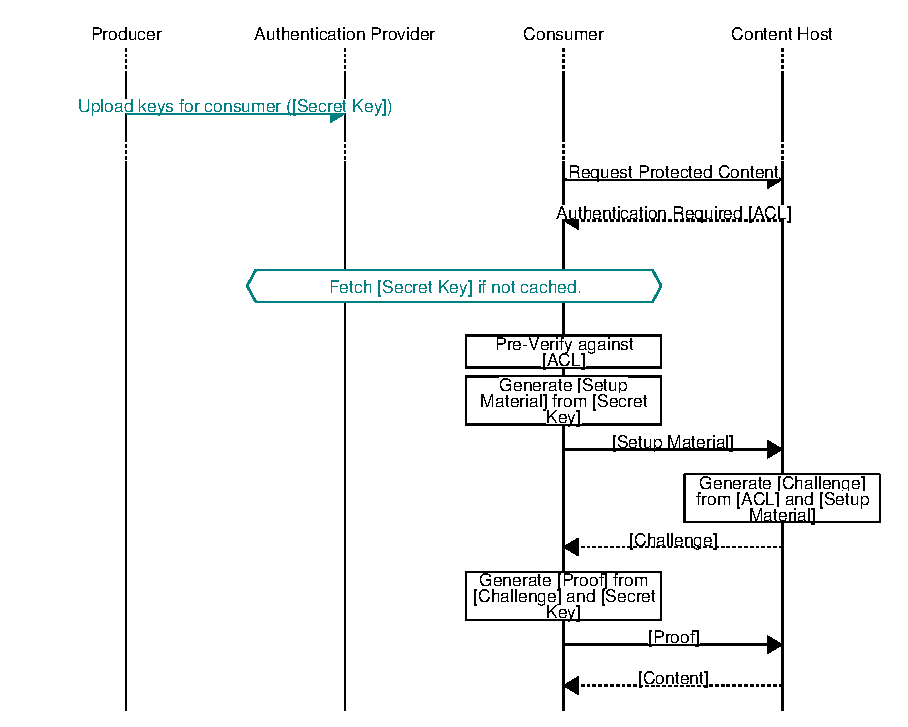
\includegraphics{auth.eps}
\end{figure}

After running this protocol, the content host learns precisely that the consumer
has chosen to authenticate against an ACL and the consumer learns the identity
of the publisher (listed in the ACL) and how many groups grant them access.

Finally, if the consumer's browser fails to generate the \verb=[Proof]=, it
warns the user. We do this to discourage content hosts from fingerprinting
consumers (see \ref{sub:fingerprinting}).

\section{Account Compromise Recovery}

There are two parts to account compromise recovery:

\begin{compactenum}
\item Account lockout.
\item Account restoration.
\end{compactenum}

To support account lockout, DRACL uses short-lived certificates (signed by the
AP) in every part of the protocol. To lock down a user's account, an AP simply
stops signing new certificates for the user in question. Unfortunately, this
won't take effect till all outstanding keys have expired (on the order of
hours).

To prevent publishers with revoked keys from gaining or granting access to
content they own, we include a short-lived certificate signed by the publisher's
AP in the ``setup material'' of the authentication protocol. To lock down an
account, the AP simply stops issuing this certificate. This will prevent anyone
from authenticating against this user's ACLs.

To prevent consumers with revoked keys from accessing content owned by other
users, we use a two-key system when authenticating against ACLs. Basically,
every ACL actually consists of two sub-ACLs: one controlled by the AP and one
controlled by the publisher. When the consumer goes to the publisher's AP to ask
for their keys, they fetch both the key controlled by the AP and the key
controlled by the publisher. This allows the publisher's AP to revoke access to
any given consumer even if the publisher never comes online. To actually revoke
a consumers keys, the consumer's AP simply stops signing them. Once their
current certificate expires, the next time the consumer attempts to fetch keys
from a publisher's APs they will be unable to present a valid certificate.

To restore an account, the AP and user work together to transition the user to a
new keypair. To do this, the user generates a new keypair and a transition
certificate signed with their old keypair. After proving their identity to the
AP (out of band), the AP also signs the transition statement and starts signing
the new keypair as usual.

After transitioning to a new key, users do not proactively replace old ACLs with
ones made with the new key as this would require additional work for content
hosts. Instead, they continue to distribute one consumer key for each keypair
ever used. While these old keys could have been compromised, we assume that the
secondary key controlled by the AP has not been so this is still secure.

\chapter{Discussion}

Above all, DRACL aims to be practical --- that is, usable in practice, not only
in theory. Additionally, DRACL aims to be secure, privacy preserving, and
developer and user friendly.

\section{Practical}

% TODO ....

\section{Secure}
\label{sub:secure}

DRACL is secure in practice. Being secure in some perfect world where all
software is perfect and bug free isn't practical. To this end, DRACL doesn't
allow unauthorized access to content (no exceptions), supports recovery from
account compromise, supports efficient revocation, discourages unauthorized
delegation of privileges, and avoids being a vector for denial of service
attacks.

Only authorized users, the publisher, and the content host are able to
access resources protected by DRACL\@. Specifically, DRACL doesn't allow the AP
to impersonate its users and access their content. A malicious AP may at most
prevent a user from accessing content they should be able to access.

Both consumers and publishers are able recover and secure compromised
accounts. We achieve this by having APs act as semi-trusted third parties that
certify their user's keys with short-term certificates. Once an AP learns that
one of its users has been compromised, it stops signing their keys. The AP then
works with the user to transition the user to a new set of keys (authenticating
the user's identity out-of-band). For a quick overview of this protocol, see
section \ref{sub:authentication}.

publishers can efficiently revoke access to content. To facilitate this,
DRACL allows users to be removed from groups without updating every ACL
mentioning the now modified group. Much of the complexity of DRACL stems from
this requirement. Unfortunately, in order to do this efficiently, we sacrificed
some security. Specifically, content published by a publisher before they
remove a consumer from a group will remain accessible to that consumer until
their publisher-specific certificate expires. We mitigate this by making
publisher-specific certificates short-lived --- they expire on the order of hours.

Consumers are discouraged from delegating access. In DRACL, we chose to do this
by making delegation all or nothing. That is, a consumer can either delegate
access to \emph{all} content shared with them by a \emph{particular publisher} or can delegate access to no content. We would prefer to make this a true
all or nothing by saying that a consumer can only delegate access to all content
of which they are authorized consumers however, this is impossible without
introducing some concept of real-world identity. A user could simply make one
``identity'' per ``friend''. \todo{Do we really care about this?}

Finally, DRACL cannot interfere with the operation of content hosts. To achieve
this, we guarantee that all DRACL operations performed by the content host will
complete in constant time. As a direct consequence of this, contents host never
initiate network requests on behalf of DRACL\@.

\section{Privacy Preserving}
\label{sec:privacy}

DRACL preserves the privacy of both publishers and consumers. Preferably,
DRACL would reveal nothing other than whether or not some user should be able to
access some resource. Unfortunately, this goal is impossible to achieve given
our efficiency constraints. However DRACL provides practically optimal privacy
given our performance constraints and some choices we've made when confronted
with unavoidable privacy/security trade-offs.

\begin{description}
\item[Everyone] The publisher is recorded in the ACL itself so the content
  host and anyone attempting to access a resource learns the identity of the
  publisher. Additionally, anyone can learn whether or not a publisher
  has put them in some group.
\item[Content Host] Content hosts know the content and learn whether or not a
  given (anonymous) consumer chooses to prove that they have access to piece of
  content.
\item[Consumers] Consumers learn whether or not they can access any resource at
  any point in time. However, they do not learn \emph{why} they have access.
  That is, they do not learn what groups they are in or what groups grant them
  access to any given resource. See section \ref{sub:practically_optimal} for some
  caveats and exceptions.
\item[Access Control Providers] access control providers learn their users
  social networks but can't act on behalf of their users and access their
  content.
\item[Publisher] An honest but curious publisher cannot learn if and
  when specific friends access their content. Given sufficient collusion and
  effort, publishers can learn something about who accesses what when but
  this is unlikely to be an issue in practice.
\end{description}

The following sections detail what various privacy leaks we do have and why.

\subsection{Practically Optimal}
\label{sub:practically_optimal}

We have three privacy leaks that aren't entirely a result of some performance or
privacy trade-off.

First, consumers can learn how many of the groups they are in allow them to
access a resource. That is, given the set of groups a consumer is in,
$\mathbb{U}$, and the set of groups that can access a resource, $\mathbb{R}$,
the consumer can learn the size of the intersection, $|\mathbb{U} \cap
\mathbb{R}|$. This is simply an artifact of the cryptographic protocol we are
using for authentication, not the result of a deliberate efficiency trade-off.

Second, anyone can learn whether or not an ACL has changed since the last time
they accessed a piece of content. In theory, one could randomize challenges so
that they look fresh every time. However this is likely more trouble
than it is worth as, for security reasons, we have content hosts present a
signed copy of the ACL along with challenges. Unfortunately, this does allow
users to prove that they have been added to or removed from a group with
certainty by learning that they have gained/lost access to content without the
ACL changing. However, regardless of what we do, consumers can learn this with
high probability, but not with certainty, by simply assuming that gaining or
loosing access to a set of content is more likely to be the result of being
added or removed from a group than the result of each of those ACLs having been
changed in a short period of time.

Third, consumers can determine a lower bound on when an ACL may have been crated
because we record the ``time'' --- technically a monotonic counter, not the
actual time --- the publisher last removed a consumer from a group before creating
an ACL in the ACL itself. This allows us to guarantee that all content published
\emph{after} a consumer is removed from a group is never accessible to that
consumer.

\subsection{The Publisher Is Public}

In DRACL, a publisher (the author of an ACL) is publicly visible in the ACL
itself. We had four options:

\begin{compactenum}
\item Make the publisher public (what DRACL does).
\item Allow users who are authorized consumers of \emph{some} content controlled
  by the publisher to learn the identity of the author.
\item Reveal the publisher to the content host only.
\item Don't reveal the publisher at all.
\end{compactenum}

It's impossible to provide guarantee 4 without sacrificing performance. In
DRACL, we avoid updating individual ACLs (we don't even contact the content
hosts) when the members of a group changes. To do this, we need to use some
additional publisher-specific information during authentication to learn if the
consumer is a member of one of the groups listed in the ACL\@. Therefore some
party participating in authentication will learn the publisher of the ACL based on
what publisher-specific information they end up using. As only the content host and
consumer are directly involved in authentication (for performance and
reliability reasons) one of those two parties will learn who the publisher is.

Providing guarantee 3 would either violate our security guarantees and open
content hosts up to denial of service attacks or force the publisher to
contact every affected content host when an ACL changes. As noted above, either
the content host or the consumer needs to learn the publisher-specific information.
To prevent the consumer from learning the identity of the publisher, we'd either
have to have the content host fetch this information from the publisher or have the
publisher send this information to the content host. The first option violates our
rule that the content host must never make network requests on behalf of DRACL\@.
As a matter of fact, this would be the worst case scenario: the content host
would be making a network request to a server specified by a client (the publisher) on behalf of a client (the consumer). On the other hand, having the publisher
send the publisher-specific information to each content host ahead-of-time would
complicate the content hosts (they would have to listen for ACL updates) and
force the publishers to contact every content host they have ever used when
they change the members of one of their groups.

If we were to provide guarantee 2, DRACL would either scale horribly at the tail
or provide dubious privacy benefit. To access a piece of content, users would
have to linearly search through a list of publisher-specific secrets from every user
who has granted them access to some piece of content. For popular users, this
list could be very large. Worse, the size of this list scales based on actions
taken by \emph{other} users, not the consumer in question. We could use a hybrid
approach where ACLs list the publisher's AP but not the publisher. This
way, consumers would only need to remember keys from publishers whose
content they frequently access; they can fetch other keys on-demand from the
listed APs. Unfortunately, the users who care about their privacy the most and
therefore run their own APs will effectively be named in their ACLs because they
are the \emph{only} user of their APs.\todo{I feel like there is a cleaner
  argument here.}

\subsection{The AP Learns The Social Network}

In DRACL, APs learn the social networks of their publishers. Specifically,
they learn the composition of their publisher's groups.

...TODO...

\subsection{Fingerprinting}
\label{sub:fingerprinting}

One problem with any access control scheme is that the content host can
fingerprint users based on what they can and cannot access. The consumer could
make every access request look like it's coming from a new client but this is
infeasible in practice. Instead DRACL allows the user to decide if and when to
authenticate (always for a content host, always for a publisher on a content
host, once, not now, never) and warns users (loudly) when authentication fails.
This way, consumers control what information they give to content hosts and
content hosts can only confirm answers they already suspect.

\subsection{Timing and Caching}

For increased performance and reliability, consumers cache keys retrieved from
publishers. Unfortunately, caching tends to leak timing information. In our
case, we were worried that a curious content host could learn whether or not a
consumer ``knew'' a publisher even if the consumer chose not to authenticate
based on whether or not the consumer had already cached the publisher's key.

To mitigate this this, consumers pre-verify (\ref{sub:authentication}) if they
will be able to access a piece of content. If this pre-verification fails, they
never even initiate the authentication protocol. This means that the content
host can only possibly learn timing information if the user has access to the
content in question and has chosen to access it. However, in this case, the
publisher already learns that the consumer ``knows'' the publisher.

\subsection{Side Channels}

Finally, they will likely learn about the consumer's browser, IP address, etc.
This is beyond the scope of DRACL system and users that require true anonymity
should use the Tor Browser\cite{tor} or Tails\cite{tails}.

\section{Developer Friendly}

To be developer friendly, DRACL wraps all content-host logic in a simple
(interface wise), environment-agnostic library.

To keep it simple, we only export three functions: \verb=is_acl=,
\verb=validate_replacement=, and \verb=authenticate=. \verb=is_acl= simply
verifies that an ACL is well formed. \verb=validate_replacement= takes an old
ACL and an ACL transition statement and returns either the new ACL that should
replace the old ACL or an error. Finally, \verb=authenticate= takes an opaque
consumer input and an opaque ACL and returns one of: \verb=GRANT=,
\verb=DENY(Reason)=, \verb=CONTINUE(OpaqueReply)= where \verb=OpaqueReply=
should be returned to the client as-is. This minimal interface should make it
easy to integrate DRACL with existing systems.

Additionally, these functions perform \emph{no} IO and run in constant time (as
noted in the security~\ref{sub:secure} section above). This significantly
reduces content host implementation complexity because it means that these
functions are environment agnostic and can be called synchronously.

Finally, access control checks never lead to database writes. This is important
for high-performance applications where reads are often performed out of
read-only caches.

\section{User Friendly}

We have designed DRACL (at the system level) to be user friendly and
unobtrusive. Specifically:

\begin{enumerate}
  \item Users only have to remember one set of credentials (their DRACL
    credentials). DRACL can even be used to sign in to other systems by treating
    accounts as resources. This, incidentally, also allows multiple people to share
    a single account without sharing passwords.
  \item Users can take their their social network with them from content host to
    content host without giving up privacy. See the related work section for a
    comparison to Facebook Connect\texttrademark~\cite{facebook-connect}
  \item Day to day, DRACL should be unobtrusive and integrate well with content
    hosts.
\end{enumerate}

These last two issues have been cited~\cite{persona-fail} by Mozilla as reasons
reasons their authentication system, Persona, failed.

\chapter{Design}

\section{Crypto}

\subsection{Setup}

%\chapter{Design}
%
%This section describes the core design and does not include concrete APIs. To
%make this design easy to follow, we'll first map the abstract publisher and
%consumer to concrete entities:
%
%\begin{compactitem}
%    \item The publisher is Penny.
%    \item The consumers are Kevin and Cary.
%\end{compactitem}
%
%Let's also assume that Penny has a stalker, Eve, who wants to see everything she
%(Penny) posts.
%
%Penny has a piece of content she wishes to share with Kevin and Cary using a
%third party service. For this story, let's say she wants to share a photo with
%Kevin and Cary using FoShare as the third party service (the content host).
%However, there's a catch: she doesn't want her stalker, Eve, to see the photo.
%Therefore, along with her photo, she needs to give FoShare some way to
%distinguish ``friend from foe''. We'll call this extra information an ACL (access
%control list). The following sections describe how this can be done.
%
%\section{``Friending''}
%
%Before they can securely share content with each other, Penny, Kevin, Cary, and
%Eve will need some way to securely and identify each other. In this system,
%they'll each use an asymmetric keypair. We will use ECC (elliptic curve
%cryptography) GnuPG keypairs as GnuPG is the de-facto decentralized PKI standard
%and elliptic curve cryptographic schemes produce very short signatures.
%
%Now that they all have unique, provable identities, they need to share these
%identities with each other so that they can talk about each other. They do this
%by exchanging public keys. This is similar to Facebook's process of friending,
%however, unlike Facebook friending, this process doesn't need to be symmetric
%and doesn't inherently give Penny, Kevin, Eve, or Cary access to each other's
%content.  We plan to use services like keybase.io~\cite{keybase} to help with
%the initial key-exchange process.
%
%Now that they can securely identify each other, Penny the publisher could just
%tell FoShare to let Kevin and Cary (the consumers) access her photo
%(identifying them by their public keys). However, this would introduce a privacy
%concern because flicker would be able to learn the identities of the two
%consumers.
%
%Instead, we use an anonymous secure group communication scheme as described in
%\cite{acp2} (based on an Access Control Polynomial (ACP) scheme described in
%\cite{acp}). ACP will allow us to efficiently encrypt a shared secret token with
%multiple secret keys without revealing anything about the secret keys. To be
%able to use ACP, Penny the publisher must first generate secret keys (called
%consumer keys) for every friend with whom she wishes to share content and
%distribute them using her AP (described in the next section).
%
%\subsection{Access Control Provider (AP)}
%
%The Access Control Provider (AP) is simply our way to deal with the fact that
%publishers and consumers aren't always online and, even when they are, they
%are often hidden behind firewalls. The AP will host consumer keys, issue
%certificates of membership (as described in the Groups and Authentication 2.0
%sections), and help both consumers and publishers generate ACLs, manage
%friend lists, authenticate, etc. Additionally, publisher and APs will share
%a ``publisher secret'' symmetric key which will be useful in the following sections.
%An AP is to DRACL as an Email Provider is to Email.
%
%For now, publishers must trust their APs to not be actively curious. That
%is, an actively curious AP can access any content owned by a publisher.
%Note, however, that publishers do not *report* the content they own to their APs so
%passively curious APs should learn nothing about their content. We may choose to
%limit AP power in the future but doing so will impact usability and performance.
%
%Finally, to make it possible for users to find their friends APs given their
%public keys, each user will list his or her AP in the UID section of his or her
%public PGP key.
%
%\todo{Explain?}
%
%\subsection{Authentication 1.0}
%
%This section describes the basic authentication protocol which we will augment
%in the Authentication 2.0 section.
%
%\subsubsection{Generating An ACL 1.0}
%
%Now that Penny has given Kevin and Cary secret keys, she can create an ACL using
%ACP\@. The ACL has three parts: a challenge, a verifier, and an encrypted
%description. The challenge includes an ACP encrypted random content token, the
%domain of the content host authorized to use this ACL, and the publisher's
%signature. The verifier is just the content token (unencrypted). The description
%is some additional data (encrypted with the publisher secret) that the publisher
%and AP can use to reconstruct the ACL\@. To keep the size of ACL within
%reasonable limits, we will, for now, limit the number of users that can be
%granted access to a particular piece of content to 150. In total, an ACL should
%be under $\unit[4]{KiB}$. In the Groups section, we will discuss methods for
%sharing content with more than 150 consumers.
%
%% NOTE: 128*150 (ACP) + 32*150 (description) + 64*8 (signature) + 128 (content
%% token) + 255*8 (content host id) == 3.3KiB (which gives us room for other stuff).
%
%\begin{figure}[H]
%\begin{minted}{JavaScript}
%{
%    challenge: {
%        data: {
%            acp: ACP(content_token, [
%                Kevin_Penny_Shared_key,
%                Cary_Penny_Shared_Key
%            ]),
%            content_host: "foshare.com"
%        },
%        publisher_signature: ECDSA(Penny_Private_Key, data),
%    },
%    verifier: content_token,
%    description: Encrypted(Penny_publisher_secret, [
%        "Kevin",
%        "Cary"
%    ])
%}
%\end{minted}
%\caption{Example ACL}
%\end{figure}
%
%
%\subsubsection{Authentication 1.0}
%
%Now Kevin learns about the photo (Penny tells him through some side channel,
%e.g.\ email) so he goes to FoShare and asks for it. However, FoShare needs to
%verify that Kevin has permission to access the photo. To do this, FoShare simply
%sends Kevin the challenge, Kevin checks Penny's signature, verifies that that
%the content host listed in the challenge is FoShare to prevent MITM attacks (we
%assume the communication channel is authenticated and encrypted with SSL),
%decrypts the ACP, and returns the content token to FoShare. FoShare then checks
%the response against its copy of the content token, and, if they match, gives
%Kevin access to the content.
%
%Now Eve tries to access the photo. From the ACL, she learns that it was
%published by Penny but that's all she learns because she is unable to decrypt
%the ACP\@. Furthermore, due to the privacy preserving nature of ACP, she is unable
%to learn anything about the members that access to the content. In the end, she
%can't access the photo because she can't recover the content token.
%
%\note{One drawback in this scheme is that, if the content host is
%compromised, all ACLs will need to be recreated. We might be able to use
%asymmetric cryptography to avoid this but that would place an additional burden
%on the content host (the ACLs would larger and the content host would have to
%check an asymmetric signature).}
%
%\subsubsection{Revoking Access 1.0}
%
%To revoke access to a piece of content, Penny simply re-creates the ACL
%associated with the content based on the encrypted description included in the
%original ACL\@.
%
%\subsection{Groups}
%
%While the scheme defined above works, it is missing a key component found in
%most access control schemes: groups. There are two primary usability benefits of
%groups:
%
%\begin{compactenum}
%    \item The ability to repeatedly grant access to a common set of consumers.
%    \item The ability to add/remove a consumer to/from the set of users able to
%        access an entire class of content.
%\end{compactenum}
%
%Unfortunately, we were unable to efficiently achieve the second usability
%benefit while preventing content hosts learning whether or not two users are in
%the same ``group''. Therefore, we have decided to introduce two types of groups:
%``cliques'' and ``organization'' (working names).
%
%\subsubsection{Cliques}
%
%In DRACL, a clique is a grouping of consumers known only to an individual
%publisher. Cliques preserve membership privacy (it's impossible for two members
%of a clique to determine whether or not they are in the same clique) however,
%new clique members will not automatically be granted access to content
%previously made available to the clique and removed clique members will retain
%access to any content made available to the clique before the member was
%removed. In short, cliques provide the first usability benefit but not the
%second.
%
%Implementation wise, cliques are simply an abstraction. When adding a clique to
%an ACL, the simply adds the members of the clique to the ACL\@. This
%trivially maintains the secrecy of clique membership.
%
%\subsubsection{Organization}
%
%An organization is analogous to a traditional POSIX group and can be used in the
%same manner. Unlike clique members, organization members gain access to all
%content ever made available to an organization when they become members and
%lose access if their memberships are revoked.
%
%Organizations are not simply an abstraction. Each organization has a publisher
%unique permanent 64bit ID\@. However, consumers never learn these IDs and content
%hosts only learn about organizations used on their service. % TODO: WORDING
%
%For example, let's say that Penny the publisher now wants to work on a her 6.824
%project with Kevin and Cary. She could just give them access to each piece of
%content individually but that would be cumbersome, especially if she needs to
%add another classmate to the project. So, instead, she creates a ``6.824
%Project'' organization and tells her AP that Kevin and Cary are members of this
%organization.
%
%Finally, we use organizations to circumvent the 150 user limit present in the
%Authentication 1.0 section. Basically, we argue that if a group contains more
%than 150 users, learning that two users are a member of the same group reveals
%relatively little to the content host beyond the fact that they know the
%publisher.
%
%\note{We chose 150 because it is Dunbar's \cite{dunbar} number. While not a hard
%limit on social group sizes, we feel this is a generous upper bound on the
%number of "close friends" a user might have.}
%
%
%
%\subsection{Authentication 2.0}
%
%In this section, we modify the authentication scheme described in Authentication
%1.0 to accommodate organizations. Organization authentication is modeled after
%kerberos~\cite{kerberos}.
%
%\subsubsection{Generating An ACL 2.0}
%
%To accommodate organizations, we include the list of organizations (obscured)
%and a shared secret for verifying membership certificates in the ACL\@.
%
%First, we include an obscured list of organizations by adding a random 16 byte
%nonce and a list of hashed (using MD5) \texttt{(nonce, organization\_id)} tuples
%to the challenge and a list of hashed (again, using MD5)
%\texttt{(content\_host\_name, organization\_ID)} to the verifier. We hash the
%organization IDs in the challenge to prevent non-members from learning anything
%about which organizations have been given access to the piece of content and we
%hash the verifier organization IDs to prevent content hosts from colluding to
%track users across services. We may additionally choose to add decoy (fake)
%organizations to obscure the cardinality. Finally, we add these organization IDs
%to the encrypted description section.
%
%\note{MD5 is sufficiently secure because we don't care about collision
%resistance.}
%
%Next, we generate a shared secret using a well-known epoch published by the  the publisher must also give the content host a
%shared secret. We use derive this secret from the publisher's secret
%(\texttt{SHA256("content host domain"|publisher secret)}) so that content hosts
%must only remember one shared secret per publisher and publishers don't have to
%remember any additional shared secrets beyond the \texttt{publisher secret}.
%
%\note{To make these ACLs ``stand alone,'' content hosts may wish to store this
%shared secret along with each ACL instead of storing it once per publisher.}
%
%
%The following is the example ACL from our story for the project's final report.
%To make this example more general, we have included an additional organization
%(``some other org'').
%
%\begin{figure}[H]
%\begin{minted}{JavaScript}
%{
%    challenge: {
%        data: {
%            nonce: some_nonce,
%            acp: ACP(content_token, []), // Empty
%            organizations: [
%                MD5(824_project|some_nonce),
%                MD5(some_other_org|some_nonce)
%            ],
%            content_host: "foshare.com"
%        },
%        publisher_signature: ECDSA(Penny_Private_Key, data),
%    },
%    verifier: {
%        content_token: content_token,
%        organizations: [
%            MD5(824_project|"foshare.com"),
%            MD5(some_other_org|"foshare.com")
%        ] 
%    },
%    description: Encrypted(Penny_publisher_secret, {
%        organizations: [824_project, some_other_org],
%        acp: []
%    })
%}
%\end{minted}
%\caption{Example ACL 2.0}
%\end{figure}
%
%\subsubsection{Learning About Organizations}
%
%Before being able to prove membership in an organization, consumers need to know
%to which organizations they belong. To learn this, they simply authenticate with
%the publisher's AP and then ask ``which organizations do I belong to?''. The AP
%responds with a list of \texttt{("Organization Name", org\_id)} tuples. In our
%example, Cary would receive the following from Penny's AP:
%\texttt{("6.824 Project", 824\_org)}.
%
%\subsubsection{Authentication 2.0}
%
%Now, to access a piece of content, the consumer can either unwrap the content
%token as described in Authentication 1.0 or prove membership in one of the
%associated organizations. Back to the example, Cary first needs to find the
%intersection between the organizations to which he belongs and the organizations
%to which Penny has granted access (to the final report). To do this, Cary,
%computes \texttt{MD5(nonce|$\text{org}_n$)} for each of Penny's organizations in
%which he is a member. He can then find the intersection between his
%organizations and the organizations listed in the ACL's challenge.
%
%Once the consumer knows the set of intersecting organizations (assuming it's
%non-empty), the browser should ask the user which, if any, organization the user
%would like to use to authenticate. Assuming the consumer decides to authenticate
%as a member of one of the organizations, he or she must then either obtain a
%certificate of membership (for that group, for a specific content host) from the
%publisher's AP or use a cached certificate. Content hosts should generally cache
%knowledge of group memberships.
%
%\note{Browsers should remember this choice and automatically authenticate with
%that organization on this content host in the future.}
%
%A certificate of membership is simply a certificate issued by the publisher's AP
%and symmetrically signed with the secret shared by the content host and the
%publisher (see the Generating an ACL 2.0 section) stating: ``The bearer of this
%certificate is a member of \texttt{MD5(content\_host\_name, organization ID)}. issued:
%\texttt{now}, expires \texttt{some time from now}.'' For example, Cary's certificate
%of membership for ``foshare.com'' would be (symmetric signature omitted):
%
%\begin{figure}[H]
%\begin{minted}{JavaScript}
%{
%    organization: MD5(824_project | "foshare.com"),
%    issued: timestamp,
%    expires: timestamp + 24h,
%}
%\end{minted}
%\caption{Example Certificate of Membership}
%\end{figure}
%
%To obtain a certificate of membership, the consumer authenticates with the
%publisher's AP and then simply asks for one. It's up to the publisher to verify
%that this consumer is a member of specified the organization.
%
%Once the consumer receives the certificate, he or she presents it to the content
%host. The content host checks the signature and, if it verifies and the
%certificate is for an acceptable organization, the content host grants access to
%the content.
%
%\note{Again, assuming a secure channel, there is no risk of a man in the middle
%attack here because this certificate is only valid at the current content host.}
%
%Back to the story, Cary wants to access the final report but is unable to
%decrypt the ACP\@. He then tries to to find an intersection between the
%organizations listed in the ACL and the ones he already knows he is a member of
%(consumers should cache organization memberships when possible to reduce the
%load on APs). As Penny just created this organization, Cary finds no
%intersection so he fetches a new list of organizations from Penny's AP and tries
%again. This time, he learns that the \texttt{824\_project} organization has access
%to the report so he obtains a certificate of membership in the group
%\texttt{824\_project} for the content host FoShare from Penny's AP
%(authenticating with his private key). He then hands this certificate over to
%FoShare which checks the certificate and finally allows Cary to access the
%document.
%
%\subsubsection{Revoking Access 2.0}
%
%Revoking access to consumers listed in the ACP is identical to the 1.0 case.
%Additionally, to revoke access to an entire organization, one simply recreates
%the ACL without that specific organization. However, safely removing a consumer
%from an organization is a bit more difficult.
%
%Simply removing a user from an organization is simple. If Penny wants to kick
%Kevin out of her 6.824 Project group, she can simply tell her AP to issue no
%more certificates of membership to Kevin. Unfortunately, this doesn't revoke
%existing certificates of membership. While they will eventually expire, they
%will remain valid for a period of time. So, while Penny can kick Kevin out
%without any issues, she can't kick Cary out so cleanly because he currently has
%a valid (``zombie'') certificate of membership (see the previous section).
%
%To reduce the impact of ``zombie'' certificates, we introduce a freshness
%constraint. Publishers record the last time they removed a member from an
%organization and, when generating an ACL for a piece of content, they tell the
%content host to not accept any certificates of membership issued before this
%time. This way consumers removed from an organization before the publisher
%gives that organization access to a piece of content will not be able to use
%their ``zombie'' certificates to access that piece of content.
%
%\note{Content hosts must be careful to include and check the issue date in
%cached group memberships information as well.}
%
%With this additional feature, Cary  will be able to continue to access old
%content made available to the organization until his certificate expires but
%will not be able to access new content. 
%
%\section{Implementation Proposal}
%
%So far, we've given a high level description of the system. This section will
%give a high level overview of how we plan to implement this system and the
%components we plan to build. Specifically, we plan to build:
%
%\begin{compactitem}
%\item Plugins for common web servers and frameworks. Specifically, we will
%    target Apache 2.0 and python based frameworks.
%\item A browser extension.
%\item A JavaScript shim library for browsers without the extension.
%    Functionality may be reduced and usability may be impacted on browsers
%    lacking the browser extension.
%\item A reference AP\@.
%\item A reference content host (FoShare).
%\end{compactitem}
%
%\subsection{Browser $\leftrightarrow$ Content-Host API}
%
%We plan on implementing two APIs for content hosts: an HTTP based API and a
%JavaScript based API\@.
%
%The HTTP based API will require browser modification (we will create an
%extension to provide the necessary functionality) but will allow for the
%cleanest integration with servers such as Apache. The HTTP based API will also
%allow us to use this protocol outside of the browser.
%
%We will implement the JavaScript API in both the browser extension and a
%shim library. The in-browser implementation will provide the best user
%experience but we will fall-back to the shim if necessary.
%
%\subsubsection{HTTP}
%
%For now, we do not plan to allow publishers to attach ACLs to content using the
%HTTP protocol. We expect they will do so by, e.g.\ writing custom
%\texttt{.htaccess} files. However, consumers will be able to authenticate over
%HTTP\@.
%
%When a consumer attempts to access content protected by an ACL, the content host
%must return an HTTP 401 Authorization Required response and include a
%\texttt{WWW-Authenticate} header with a URL where the DRACL challenge may be
%found. The consumer should then download the challenge (by issuing a GET
%request), generate a response (see Authentication 2.0), and then repeat the
%original request, this time with an \texttt{Authorization} header containing the
%response to the challenge.
%
%Unfortunately, this scheme requires an additional GET request to fetch the
%challenge because the challenge may be too large to comfortably fit in
%\texttt{WWW-Authenticate} header.
%
%\subsubsection{JavaScript}
%
%The JavaScript API will provide the following methods:
%
%\begin{minted}{JavaScript}
%// Ask a consumer to prove that he or she is authorized to
%// access a piece of content.
%function DRACLAuthenticate(challenge, callback);
%
%// Ask a publisher to create a ACL for the described content.
%// The `contentDescription` argument is a short plain-text
%// description of the content.
%function DRACLCreateACL(contentDescription, callback);
%
%// Ask a publisher to update an ACL\@. The `aclDescription`
%// argument is the description from the ACL itself.
%function DRACLUpdateACL(contentDescription, aclDescription, callback);
%\end{minted}
%
%\subsection{Browser $\leftrightarrow$ Access Control Provider API}
%
%This document will not discuss the specifics of the API for communication
%between consumers, publishers, and APs. While important, the design of this API
%will be driven by implementation needs and is not an API that can be reasonably
%designed in advance. Additionally, this API will only impact browser authors and
%Access Control Providers so, while important, it doesn't have to be elegant.
%
%\subsection{Web Server Plugin APIs}
%
%We will target python based frameworks by building a simple library that
%provides the following two methods:
%
%\begin{minted}{python}
%def create_challenge(ACL):
%    """Returns the challenge field of the ACL\@."""
%    # ...
%
%def check_challenge(ACL, response):
%    """Returns true iff the response is validates."""
%    # ...
%\end{minted}
%
%We will target Apache 2.0 by providing a server plugin and integrating with
%\texttt{.htaccess}.
%
%\section{Discussion}
%
%\subsection{Availability}
%
%This system never requires that the publisher/consumer be online at the same
%time. Both the consumer and producer will be able to use the system from behind
%firewalls.
%
%This system does require that the Access Control Provider be available most of
%the time but can tolerate small windows of down-time. % TODO: Explain?
%
%\subsection{Performance}
%
%\subsubsection{Access Control Provider}
%
%The communication overhead for the Access Control Provider are no worse than
%Kerberos. Consumers will re-use their secret keys so they will only have to
%communicate with Access Control Providers to retrieve organization membership
%certificates. As this organization certificate system is modeled after Kerberos,
%its performance characteristics should be similar.
%
%Producers only need to contact their Access Control Providers when modifying their
%friend-list so the \emph{overhead} should be zero. That is, managing a
%friend-list always requires communication and DRACL doesn't add any additional
%communication requirements.
%
%The storage overheads per user are:
%
%\begin{compactitem}
%\item 1 Elliptic Curve Key Key Pair ($\unit[256]{bits}$)
%\item 1 Publisher Secret ($\unit[256]{bits}$)
%\item Two shared secrets per friend (assuming bi-directional friendship)
%    ($\unit[128]{bits}$ each, estimated 300 friends per user = $\unit[9.36]{KiB}$)
%    % TODO: shared secret too small?
%\item Organization IDs ($\unit[64]{bits}$ each, estimated 10 per user = $\unit[70]{KiB}$).
%\end{compactitem}
%
%Conservatively, no Access Control Provider should have to store more than
%$\unit[100]{KiB}$ (including miscellaneous metadata) per user.
%
%The cryptographic overhead is minimal. The Access Control Provider must verify
%an ECDSA signature to authenticate consumers once per ``session'' but can cache
%a user's identity using a cookie (TBD). The AP must also compute one symmetric
%signature per organization membership certificate issued but this overhead will
%quickly be dwarfed by whatever crypto is used to secure the communication
%channel.
%
%\subsubsection{Content Host}
%
%Facebook users publish 2.5 Million pieces of content per day on average in 2012
%(about $\unit[500]{TB}$ of data)~\cite{fbnum}. This is about $\unit[195]{KiB}$
%per piece of content so a $\unit[4]{KiB}$ overhead won't hurt too much ($2\%$
%overhead).
%
%On the other hand, tweets have an upper limit of 140 bytes so a $\unit[4]{KiB}$
%overhead means that issuing per-tweet ACL's will lead to a $2826\%$ minimum
%overhead. This will bump Twitter's data storage requirements up from
%$\unit[65]{GiB}$ per day to $\unit[2]{TiB}$ per day (based on a 500 million
%tweets per day claim made by twitter\cite{twitter}. Unfortunately, ECDSA
%signatures themselves take 64 bytes so we're stuck with a $50\%$ overhead per
%tweet from the signature alone (and ECDSA signatures are some of the shortest
%around \cite{todo}). Therefore, I feel that per-tweet ACLs are simply
%infeasible.
%
%Currently, all of these storage overheads translate directly into communication
%overheads. We could support sending partial ACL challenges however, this just
%isn't worth the trouble. Even when using ACL's large enough to support 1200
%independent ACP entries (8 times the current size), batching 20 resource
%requests together to reduce the effects of latency, and splitting ACL's 16 ways,
%ACL splitting only yields a 6x speedup (assuming $\unit[50]{ms}$ network
%latencies and the world-wide bandwidth average of
%$\unit[3.6]{Mbps}$~\cite{akamai}). Once the bandwidth is bumped up to the FCC's
%broadband definition ($\unit[25]{Mbps}$)~\cite{fcc} the speedup drops to 1.5x.
%
%Again, the cryptographic overhead is minimal. The content host may have to
%verify a single symmetric signature per piece of content accessed (the
%pathological worst case scenario where each piece of content has been published
%to a different organization). However, this overhead should again be dwarfed by
%the overhead of the crypto used to secure the communication channel.
%
%\subsection{Security Concerns}
%
%\subsubsection{Access Delegation}
%
%The primary security issue in this system is access delegation. That is,
%consumers can delegate their access to content either intentionally or
%unintentionally (due to a security breach).
%
%A consumer can indefinitely delegate (give away) access to all content shared
%with him or her by a single friend by giving away his or her shared secret. We
%hope that giving away access to everything will be enough to prevent them from
%doing so willingly.
%
%A consumer can temporarily give another user access to resources published to an
%organization by giving away his or her membership certificate. Fortunately, this
%fine-grained delegation is only possible for short periods of time because these
%certificates expire.
%
%The biggest concern is what happens if an attacker steals a user's credentials.
%Currently, there is nothing we can do to recover.
%
%\subsection{Privacy}
%
%The content host can map users to host-specific organization identifiers and
%colluding users can determine if they are in the same organization. However, for
%small groups (Cliques), group membership is completely hidden.
%
%\subsection{Usability}
%
%This protocol should be very easy for content hosts to implement. From the
%content-host's perspective, the authentication mechanism is stateless.
%Furthermore, the content-host never needs to contact the Authentication Agent
%when authenticating which means that the server-side DRACL code can be
%sandboxed.

% TODO

%* Handling Security Compromises
%
%  - Relying Agent (replacing compromised ACLs)
%
%  - Consumers
%
%  - Publishers
%
%* Remove users from groups.
%
%* Prevent group members from permanently delegating privileges.
%
%* Safely using credentials on untrusted hardware.
%
%* Syncing and Backing up credentials between machines.
%
%* Avoid creating one-off groups (multiple groups in an ACL).
%
%* A distributed key distribution system.
%
%* Make it possible to decrypt an {encrypted token} without trying every group
%  known key.
%
%* Prevent MITM\@. Currently, Kevin must trust that FoShare isn't actually Eve in
%  disguise.
%
%
%# Key distribution service.

\bibliographystyle{acm}
\bibliography{thesis}

\end{document}
% vim: set foldmethod=marker: %
